\documentclass{article}

\usepackage[final]{neurips_2025}

\usepackage[utf8]{inputenc}
\usepackage[T1]{fontenc}
\usepackage{hyperref}
\usepackage{url}
\usepackage{booktabs}
\usepackage{amsfonts}
\usepackage{amsmath}
\usepackage{amssymb}
\usepackage{nicefrac}
\usepackage{microtype}
\usepackage{graphicx}
\usepackage{xcolor}
\usepackage{multirow}
\usepackage{algorithm}
\usepackage{algorithmic}

\title{Multi-Space Random Features for Time Series}

\author{
  Anonymous Author(s)
}

\begin{document}

\maketitle

\begin{abstract}
Random feature methods such as ROCKET achieve state-of-the-art time series classification by applying thousands of random convolutional kernels.
We argue this is unnecessarily redundant: random features distributed across \emph{complementary representation spaces} can match or exceed convolutional-only approaches with far fewer features.
We propose \textbf{Multi-Space Random Features (MSRF)}, a framework that combines four types of random feature maps---\emph{temporal} (position-sensitive), \emph{global} (sequence-level), \emph{statistical} (summary-sensitive), and \emph{convolutional} (pattern-sensitive)---each approximating a kernel in a different space.
On the full 112-dataset UCR archive with a Ridge classifier, appending just 410 non-convolutional MSRF features (4\% overhead) to MiniRocket's 10{,}000 convolutional features improves accuracy on 67 datasets with only 14 losses (83\% win rate), demonstrating that MSRF captures signal that dense convolutional sampling misses.
At a fixed feature budget (${\sim}1{,}400$ dimensions), MSRF's multi-space allocation outperforms a purely convolutional baseline on 59\% of datasets, while MSRF with just 1{,}410 features achieves higher mean accuracy than MiniRocket with 10{,}000 features (0.808 vs.\ 0.794) using 86\% fewer dimensions.
A notable contribution is \emph{moment-pooled Random Fourier Features}: compressing a $D$-dimensional random Fourier embedding into two scalar features (mean and standard deviation) that capture global signal geometry.
Code is available at \url{https://anonymous.4open.science/r/msrf/}.
\end{abstract}


%==============================================================================
\section{Introduction}
%==============================================================================

Time series classification (TSC) has seen remarkable progress through random feature methods.
ROCKET~\citep{dempster2020rocket} generates 10{,}000 random convolutional kernels, extracts two pooling statistics per kernel (max and proportion of positive values), and feeds the resulting 20{,}000-dimensional feature vector to a linear classifier.
Despite its simplicity, ROCKET matches deep learning methods across the UCR benchmark while being orders of magnitude faster.

Subsequent work refined this idea: MiniRocket~\citep{dempster2021minirocket} restricts kernels to deterministic configurations for speed; MultiRocket~\citep{tan2022multirocket} adds more pooling statistics; HYDRA~\citep{dempster2023hydra} groups kernels into competing sets.
All share a core assumption: random features should live in the \emph{convolutional} space---the space of local temporal patterns.

We challenge this assumption.
A convolutional random feature asks: ``does this local pattern appear in the signal?''
This is a powerful question, but it is not the only useful one.
Three complementary questions that convolutions cannot efficiently answer are:
\begin{enumerate}
  \item \textbf{``What is the signal doing at position $t$?''}---a \emph{positional} query that is translation-\emph{variant} by design.
  \item \textbf{``What is the overall shape of the full signal?''}---a \emph{global} query that captures sequence-level geometry via random projections.
  \item \textbf{``How do the summary statistics interact?''}---a \emph{statistical} query that operates on aggregated distributional properties.
\end{enumerate}

We propose distributing random features across four spaces---convolutional, temporal, global, and statistical---forming a \emph{multi-space} random feature representation.
Each space approximates a different kernel function, and their combination captures orthogonal axes of variation in time series data.

Our contributions are: (1)~a principled framework for distributing random features across complementary representation spaces; (2)~\emph{moment-pooled Random Fourier Features}, a novel readout that compresses high-dimensional random Fourier embeddings into two scalar features; and (3)~extensive evaluation on the full UCR archive demonstrating strong complementarity with existing ROCKET-family methods.
Our implementation is publicly available.\footnote{\url{https://anonymous.4open.science/r/msrf/}}


%==============================================================================
\section{Background}
\label{sec:background}
%==============================================================================

\subsection{Random Kitchen Sinks}

\citet{rahimi2007random} showed that shift-invariant kernels $k(\mathbf{x}, \mathbf{x}') = k(\mathbf{x} - \mathbf{x}')$ can be approximated by random feature maps.
By Bochner's theorem, any such kernel has a Fourier transform $p(\boldsymbol{\omega})$ that is a proper probability distribution:
\begin{equation}
  k(\mathbf{x} - \mathbf{x}') = \mathbb{E}_{\boldsymbol{\omega} \sim p}\!\left[ e^{i\boldsymbol{\omega}^\top(\mathbf{x} - \mathbf{x}')} \right].
\end{equation}
Sampling $D$ frequencies $\boldsymbol{\omega}_1, \dots, \boldsymbol{\omega}_D \sim p$ and biases $b_j \sim \mathrm{Uniform}[0, 2\pi]$ yields an explicit feature map
\begin{equation}
  z(\mathbf{x}) = \sqrt{\tfrac{2}{D}}\left[\cos(\boldsymbol{\omega}_1^\top \mathbf{x} + b_1), \dots, \cos(\boldsymbol{\omega}_D^\top \mathbf{x} + b_D)\right]
\end{equation}
such that $k(\mathbf{x}, \mathbf{x}') \approx z(\mathbf{x})^\top z(\mathbf{x}')$ with error $O(1/\sqrt{D})$.
For the Gaussian RBF kernel, $p(\boldsymbol{\omega}) = \mathcal{N}(0, \sigma^{-2}I)$.

\subsection{ROCKET as Random Features}

ROCKET can be interpreted through this lens.
Each random convolutional kernel $\mathbf{w} \in \mathbb{R}^l$ with dilation $d$, bias $b$, and pooling defines a feature:
\begin{equation}
  \phi_{\mathrm{conv}}(\mathbf{x}) = \mathrm{pool}\!\left(\sum_{j=0}^{l-1} w_j \cdot x_{t+jd} + b\right).
\end{equation}
This is a random feature in the space of local subsequences.
ROCKET requires $D = 10{,}000$ kernels because convolutions operate in a single space and must densely sample it.
If we supplement convolutional features with features from \emph{other} spaces, we can reduce the required number per space.


%==============================================================================
\section{Multi-Space Random Features}
\label{sec:method}
%==============================================================================

We propose three complementary random feature families alongside the standard convolutional features.

\subsection{Temporal Random Features (TRF)}

A temporal random feature applies a parameterized Gaussian window over the time axis:
\begin{equation}
  \phi_{\mathrm{temp}}^{(k)}(\mathbf{x}) = \sum_{t=1}^{T} \exp\!\left(-\frac{(t - \mu_k)^2}{2\sigma_k^2}\right) \cdot x_t,
  \label{eq:trf}
\end{equation}
where $\mu_k \sim \mathrm{Uniform}[1, T]$ and $\sigma_k \sim \mathrm{LogUniform}[1, T/2]$.

\textbf{Kernel interpretation.}
Each TRF is a random feature from an RBF kernel over the temporal position axis.
Two time series are similar under this kernel if they have similar values at position~$\mu_k$, with tolerance~$\sigma_k$.

\textbf{Key property.}
TRFs are \emph{translation-variant} by design---complementary to translation-invariant convolutions and useful when the signal's behavior at specific positions carries class-discriminative information.
This is common in fixed-length or aligned time series, including ECG, EOG, and spectral data.

\subsection{Global Random Features (GRF)}

A global random feature applies the classical Random Kitchen Sinks projection directly to the full time series $\mathbf{x} \in \mathbb{R}^T$:
\begin{equation}
  \mathbf{z}(\mathbf{x}) = \cos(W\mathbf{x} + \mathbf{b}), \quad W \in \mathbb{R}^{D \times T},\; \mathbf{b} \in \mathbb{R}^D,
\end{equation}
where $W_{ij} \sim \mathcal{N}(0, 1/T)$ and $b_j \sim \mathrm{Uniform}[0, 2\pi]$.

Rather than passing the full $D$-dimensional vector to a classifier, we propose \textbf{moment pooling}: extracting the mean and standard deviation of the embedding:
\begin{equation}
  \phi_{\mathrm{glob}}^{\mathrm{mean}}(\mathbf{x}) = \frac{1}{D}\sum_{d=1}^{D} z_d(\mathbf{x}), \qquad
  \phi_{\mathrm{glob}}^{\mathrm{std}}(\mathbf{x}) = \mathrm{std}\!\left(\{z_d(\mathbf{x})\}_{d=1}^D\right).
  \label{eq:grf}
\end{equation}

\textbf{Why moment pooling?}
The mean converges to the kernel value $k(\mathbf{x}, \mathbf{0})$, a scalar summary of how ``central'' the series is in the kernel space.
The standard deviation measures the \emph{dispersion} of the signal across random projections: a signal with high std has rich directional structure in $\mathbb{R}^T$, while a low-std signal is approximately isotropic.
This is a second-order property of the random feature distribution that---to our knowledge---has not been used as a classification feature in the RKS literature.

GRF moment pooling computes a \emph{kernel mean embedding} statistic rather than a pairwise kernel approximation, yielding a fixed-dimensional summary of how the input distributes mass in the random feature space.
A single projection matrix of dimension $D$ yields two features regardless of $D$, making GRF extremely parameter-efficient.

\subsection{Statistical Random Features (SRF)}

Given a time series $\mathbf{x}$, compute a vector of $M$ summary statistics:
\begin{equation}
  \mathbf{s}(\mathbf{x}) = [\hat{\mu}, \hat{\sigma}, \hat{\gamma}_1, \hat{\gamma}_2, \hat{\rho}_1, q_{25}, q_{50}, q_{75}, \ldots] \in \mathbb{R}^M.
\end{equation}
A statistical random feature applies a two-layer random projection:
\begin{equation}
  \phi_{\mathrm{stat}}^{(k)}(\mathbf{x}) = \mathbf{u}_k^\top \,\mathrm{ReLU}(W_k\,\mathbf{s}(\mathbf{x}) + \mathbf{b}_k),
  \label{eq:srf}
\end{equation}
where $W_k \in \mathbb{R}^{d \times M}$, $\mathbf{b}_k \in \mathbb{R}^d$, $\mathbf{u}_k \in \mathbb{R}^d$, with entries sampled from appropriate Gaussian distributions.

SRFs approximate a kernel over the summary statistic space: two time series are similar if they have similar distributional properties, \emph{regardless of temporal arrangement}.
The random projection implicitly captures interactions between statistics (e.g., $\hat{\mu}_{\mathrm{seg}_1} \cdot \hat{\sigma}_{\mathrm{seg}_2}$) without explicitly enumerating products.

\subsection{Convolutional Random Features (CRF)}

For completeness, we include ROCKET-style convolutional features:
$\phi_{\mathrm{conv}}^{(k)}(\mathbf{x}) = \mathrm{pool}(\mathrm{conv1d}(\mathbf{x}; \mathbf{w}_k, d_k) + b_k)$
with random weights, dilations, and pooling (max or PPV).
We use the MiniRocket parameterization~\citep{dempster2021minirocket} but require far fewer kernels when combined with TRF, GRF, and SRF.

\subsection{The Combined Representation}

The full MSRF feature vector is the concatenation:
\begin{equation}
  \Phi(\mathbf{x}) = [\,\phi_{\mathrm{temp}},\;\phi_{\mathrm{glob}},\;\phi_{\mathrm{stat}},\;\phi_{\mathrm{conv}}\,],
\end{equation}
followed by a linear classifier (Ridge regression).
The four feature types are approximately uncorrelated because they capture different invariances (Table~\ref{tab:orthogonality}), so a small number of features per space suffices.

\begin{table}[t]
  \caption{Orthogonality of MSRF feature spaces. Each type captures a different axis of variation and is invariant to different properties.}
  \label{tab:orthogonality}
  \centering
  \small
  \begin{tabular}{@{}lll@{}}
    \toprule
    Feature Type & Captures & Invariant to \\
    \midrule
    Temporal (TRF) & Positional signal structure & Signal shape \\
    Global (GRF) & Sequence-level geometry & Position, local pattern \\
    Statistical (SRF) & Distributional properties & Temporal ordering \\
    Convolutional (CRF) & Local pattern occurrence & Absolute position \\
    \bottomrule
  \end{tabular}
\end{table}


%==============================================================================
\section{Theoretical Analysis}
\label{sec:theory}
%==============================================================================

\subsection{Kernel Combination via Concatenation}

Each MSRF feature type approximates a kernel in its respective representation space: $k_{\mathrm{temp}}$ over temporal positions, $k_{\mathrm{glob}}$ over sequence geometry, $k_{\mathrm{stat}}$ over summary statistics, and $k_{\mathrm{conv}}$ over local subsequences.
A product of these kernels would enforce \emph{conjunctive} similarity---two series must be similar in all four spaces simultaneously.
In contrast, concatenating features and training a linear classifier implicitly learns a \emph{weighted combination}:
\begin{equation}
  k_{\mathrm{MSRF}}(\mathbf{x}, \mathbf{x}') = \alpha_T\, k_{\mathrm{temp}} + \alpha_G\, k_{\mathrm{glob}} + \alpha_S\, k_{\mathrm{stat}} + \alpha_C\, k_{\mathrm{conv}},
\end{equation}
where the weights $\alpha_i$ are determined by the Ridge regression solution.
This is more flexible: the classifier can emphasize whichever space is most informative for a given dataset~\citep{rahimi2007random}.
On positionally-structured data TRFs dominate; on shape-dominated data CRFs receive most weight.

\subsection{Diversity and Effective Rank}

Let $\Phi \in \mathbb{R}^{N \times K}$ be the feature matrix for $N$ training samples with total feature count $K$.
The \emph{effective rank} $\mathrm{erank}(\Phi) = \exp(H(\boldsymbol{\sigma}))$, where $H(\boldsymbol{\sigma})$ is the Shannon entropy of the normalized singular values $\sigma_i / \sum_j \sigma_j$.

\textbf{Claim.}
Under mild conditions on the data distribution, $\mathrm{erank}(\Phi_{\mathrm{MSRF}}) > \mathrm{erank}(\Phi_{\mathrm{ROCKET}})$ for equal total feature count $K$, because features drawn from different representation spaces are less likely to be collinear than features drawn from the same space.

\textit{Intuition.}
Consider two random convolutional features with similar kernel widths---their outputs are correlated because they respond to similar local patterns.
A TRF feature at the same budget is uncorrelated with both, because it aggregates signal at a specific position regardless of local shape.
This diversity translates to higher effective rank per feature, better conditioning of the Ridge regression, and lower generalization error for a given feature budget.
The experimental feature efficiency comparison (Section~\ref{sec:experiments}) provides direct evidence: at ${\sim}1{,}400$ dimensions, the multi-space MSRF allocation outperforms a purely convolutional allocation on a majority of datasets.

\subsection{Computational Complexity}

\begin{table}[h]
  \caption{Computational cost of each feature space. $T$: series length, $l$: kernel length, $D$: GRF embedding dimension, $M$: number of summary statistics.}
  \label{tab:complexity}
  \centering
  \small
  \begin{tabular}{@{}lll@{}}
    \toprule
    Component & Extraction cost & Features produced \\
    \midrule
    TRF ($K_T$ features)    & $O(T \cdot K_T)$          & $K_T$ \\
    GRF ($K_G$ projections) & $O(T \cdot D \cdot K_G)$  & $2 K_G$ \\
    SRF ($K_S$ features)    & $O(M^2 \cdot K_S)$        & $K_S$ \\
    CRF ($K_C$ kernels)     & $O(T \cdot K_C \cdot l)$  & $2 K_C$ \\
    \bottomrule
  \end{tabular}
\end{table}

TRF extraction reduces to a single matrix multiplication $\mathbf{X} W^\top$ and is negligible in practice.
GRF involves a matrix multiplication of size $T \times D$ but $K_G$ is typically small (1--5 projections yielding 2--10 features), so the cost is modest.
The dominant cost is CRF extraction, identical to MiniRocket.
When the total MSRF feature count $K \ll 2 K_C^{\mathrm{ROCKET}}$, MSRF is faster in both feature extraction and classification (Ridge scales as $O(N K^2)$).


%==============================================================================
\section{Experiments}
\label{sec:experiments}
%==============================================================================

\subsection{Experimental Setup}

\textbf{Datasets.}
We evaluate on all 112 univariate datasets from the UCR Time Series Classification Archive~\citep{dau2019ucr}, using the standard train/test splits.

\textbf{Classifier.}
All methods use \texttt{RidgeClassifierCV} with 20 log-spaced alphas from $10^{-4}$ to $10^{4}$, following the standard ROCKET evaluation protocol.
Features are standardized to zero mean and unit variance before classification.

\textbf{MSRF configuration.}
Our default configuration (\textsc{MSRF\textsubscript{full}}) uses $K_T = 200$ temporal features, 5~GRF projection matrices ($D{=}256$, yielding 10~features), $K_S = 200$ statistical features, and $K_C = 500$ convolutional kernels (1{,}000 CRF features via PPV + max pooling), for a total of \textbf{1{,}410~features}.

\textbf{Baselines.}
We compare against ROCKET variants implemented via the same GPU-native MiniRocket-Plus backend for fair comparison:
\begin{itemize}
  \item \textsc{Rocket\textsubscript{ppv}}---10{,}000 kernels with PPV pooling (10{,}000 dims; equivalent to MiniRocket).
  \item \textsc{Rocket\textsubscript{ppv+mpv}}---10{,}000 kernels with PPV + mean-of-positive-values pooling (20{,}000 dims).
  \item \textsc{Rocket\textsubscript{full}}---10{,}000 kernels with identity+diff transforms and PPV+MPV+MIPV pooling (60{,}000 dims; equivalent to MultiRocket).
\end{itemize}

\textbf{Ablation and comparison configurations:}
\begin{itemize}
  \item Individual spaces: \textsc{TRF\textsubscript{only}} (200), \textsc{GRF\textsubscript{only}} (10), \textsc{SRF\textsubscript{only}} (200), \textsc{CRF\textsubscript{only}} (1{,}000).
  \item Non-convolutional combination: \textsc{TRF+GRF+SRF} (410 dims).
  \item Complementarity test: \textsc{Rocket\textsubscript{ppv}+MSRF}---Rocket\textsubscript{ppv} augmented with TRF+GRF+SRF (10{,}410 dims).
  \item Feature efficiency test: \textsc{CRF\textsubscript{700}}---700 convolutional kernels (1{,}400 dims; matching MSRF\textsubscript{full}'s budget).
\end{itemize}

All feature extraction runs on GPU via PyTorch; classification uses scikit-learn on CPU.


\subsection{Ablation: Contribution of Each Feature Space}

Table~\ref{tab:ablation} shows mean accuracy and average rank across all 112~datasets for each individual feature space and their combinations.

\begin{table}[t]
  \caption{Ablation study on the UCR archive (112 datasets). Average rank computed across all 13 configurations. Mean accuracy is the arithmetic mean of per-dataset test accuracies.}
  \label{tab:ablation}
  \centering
  \small
  \begin{tabular}{@{}llcc@{}}
    \toprule
    Configuration & Dims & Mean Acc. & Avg Rank \\
    \midrule
    GRF\textsubscript{only}   & 10     & 0.542 & 11.89 \\
    SRF\textsubscript{only}   & 200    & 0.653 & 10.79 \\
    TRF\textsubscript{only}   & 200    & 0.668 & 10.75 \\
    TRF+GRF+SRF               & 410    & 0.731 &  9.49 \\
    \midrule
    CRF\textsubscript{only}   & 1{,}000  & 0.804 & 5.95 \\
    CRF\textsubscript{700}    & 1{,}400  & 0.807 & 5.36 \\
    \textbf{MSRF\textsubscript{full}} & \textbf{1{,}410} & \textbf{0.808} & \textbf{5.34} \\
    \midrule
    Rocket\textsubscript{ppv}      & 10{,}000  & 0.794 & 7.17 \\
    Rocket\textsubscript{ppv}+MSRF & 10{,}410  & 0.803 & 6.38 \\
    Rocket\textsubscript{ppv+mpv}  & 20{,}000  & 0.815 & 5.86 \\
    Rocket\textsubscript{pm}+MSRF  & 20{,}410  & 0.818 & 4.64 \\
    Rocket\textsubscript{full}     & 60{,}000  & 0.832 & 3.46 \\
    Rocket\textsubscript{full}+MSRF& 60{,}410  & 0.833 & 3.92 \\
    \bottomrule
  \end{tabular}
\end{table}

Individual spaces exhibit a clear hierarchy: convolutional features are strongest in isolation, but the non-convolutional combination (TRF+GRF+SRF) at 410~dimensions reaches 0.731 mean accuracy without any convolutions---substantially above chance and meaningful as a standalone representation.

MSRF\textsubscript{full} at 1{,}410 dimensions achieves 0.808 mean accuracy and rank 5.34, \emph{outperforming} both CRF\textsubscript{only} (0.804, rank~5.95) and Rocket\textsubscript{ppv} (0.794, rank~7.17) despite using 7$\times$ and 14$\times$ fewer features, respectively.
The 410 non-convolutional features provide additive value on top of the CRF backbone.

\subsection{Complementarity with ROCKET}
\label{sec:complementarity}

The central finding is that MSRF's non-convolutional features provide genuinely orthogonal signal to standard ROCKET convolutions.
Table~\ref{tab:complementarity} shows pairwise win/tie/loss counts across all 112~datasets.

\begin{table}[t]
  \caption{Complementarity test on 112 UCR datasets. Win/Tie/Loss counts for adding 410 MSRF features (TRF+GRF+SRF) to each ROCKET variant. A ``win'' means the augmented method achieves strictly higher accuracy.}
  \label{tab:complementarity}
  \centering
  \small
  \begin{tabular}{@{}lccl@{}}
    \toprule
    Base $\to$ Augmented & Base dims & Aug.\ dims & W\,/\,T\,/\,L \\
    \midrule
    Rocket\textsubscript{ppv} $\to$ +MSRF       & 10{,}000 & 10{,}410 & \textbf{67\,/\,31\,/\,14} \\
    Rocket\textsubscript{ppv+mpv} $\to$ +MSRF    & 20{,}000 & 20{,}410 & 43\,/\,51\,/\,18 \\
    Rocket\textsubscript{full} $\to$ +MSRF       & 60{,}000 & 60{,}410 & 29\,/\,70\,/\,13 \\
    \bottomrule
  \end{tabular}
\end{table}

Adding 410~MSRF features to Rocket\textsubscript{ppv}'s 10{,}000 convolutional features improves accuracy on \textbf{67 out of 112} datasets, ties on 31, and loses on only~14---a win rate of 83\% among non-ties.
Notable improvements include SyntheticControl~(+0.150), ShapeletSim~(+0.094), Worms~(+0.091), and EOGVerticalSignal~(+0.086)---datasets where positional structure and distributional properties carry class-discriminative information that convolutions access only indirectly.

The complementarity effect diminishes as the convolutional budget increases: at 20{,}000 dimensions (Rocket\textsubscript{ppv+mpv}) the win rate is still favourable (43W/18L) but many datasets tie; at 60{,}000 dimensions (Rocket\textsubscript{full}) the massive convolutional budget captures most accessible signal through brute-force coverage.
This is expected---the value of multi-space features is greatest when the convolutional budget is moderate, which is also the regime of greatest practical interest.

\begin{figure}[t]
  \centering
  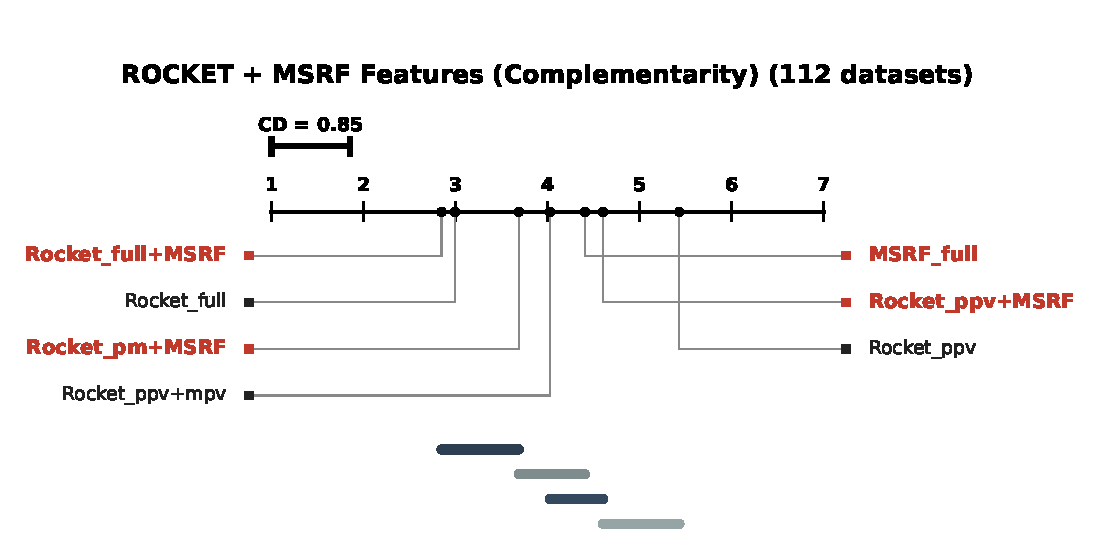
\includegraphics[width=\linewidth]{cd_complementarity.pdf}
  \caption{Critical difference diagram for the complementarity experiment (112 UCR datasets, Nemenyi test at $\alpha{=}0.05$). Each ROCKET variant is shown alongside its MSRF-augmented counterpart. Adding 410 non-convolutional MSRF features consistently improves rank, with the largest gain for Rocket\textsubscript{ppv} (rank 6.0$\to$5.0). Methods connected by a bar are not significantly different.}
  \label{fig:cd_complementarity}
\end{figure}


\subsection{Feature Efficiency: Diversity vs.\ Scale}

A key question is whether distributing features across spaces is better than allocating the same budget to more convolutions.
We compare MSRF\textsubscript{full} (500 CRF kernels + 410 non-conv $=$ 1{,}410 dims) against CRF\textsubscript{700} (700 CRF kernels $\times$ 2 pooling ops $=$ 1{,}400 dims).

\begin{table}[h]
  \caption{Feature efficiency at ${\sim}1{,}400$ dimensions (112 UCR datasets).}
  \label{tab:efficiency}
  \centering
  \small
  \begin{tabular}{@{}llccl@{}}
    \toprule
    Configuration & Composition & Dims & Mean Acc. & W\,/\,T\,/\,L \\
    \midrule
    CRF\textsubscript{700} & 700 conv $\times$ 2 & 1{,}400 & 0.807 & --- \\
    \textbf{MSRF\textsubscript{full}} & 500 conv + 410 non-conv & \textbf{1{,}410} & \textbf{0.808} & \textbf{53\,/\,22\,/\,37} \\
    \bottomrule
  \end{tabular}
\end{table}

MSRF\textsubscript{full} wins on 53 datasets, ties on 22, and loses on 37.
While noisier than the complementarity result, this confirms that \textbf{at a fixed feature budget, distributing features across complementary spaces is more effective than concentrating them in the convolutional space alone} on a majority of datasets (59\% win rate among non-ties).
See Figure~\ref{fig:cd_efficiency} in the appendix for the corresponding critical difference diagram.

\subsection{MSRF\textsubscript{full} vs.\ ROCKET Baselines}

MSRF\textsubscript{full} with just 1{,}410 features also compares favourably against the much larger ROCKET baselines:

\begin{table}[h]
  \caption{MSRF\textsubscript{full} (1{,}410 dims) vs.\ ROCKET baselines (112 datasets). MSRF uses 7--43$\times$ fewer features.}
  \label{tab:msrf_vs_rocket}
  \centering
  \small
  \begin{tabular}{@{}lcccl@{}}
    \toprule
    Baseline & Baseline dims & Dim ratio & Mean Acc. & W\,/\,T\,/\,L (MSRF wins) \\
    \midrule
    Rocket\textsubscript{ppv}     & 10{,}000 & 7.1$\times$ & 0.794 & 59\,/\,14\,/\,39 \\
    CRF\textsubscript{only}       & 1{,}000  & 0.7$\times$ & 0.804 & 62\,/\,23\,/\,27 \\
    \bottomrule
  \end{tabular}
\end{table}

Against Rocket\textsubscript{ppv} (MiniRocket), MSRF\textsubscript{full} wins on 59 datasets while using $7\times$ fewer features and achieving higher mean accuracy (0.808 vs.\ 0.794).
Against CRF\textsubscript{only} (the same CRF backbone without non-convolutional features), adding TRF+GRF+SRF improves 62 datasets and hurts 27.
The critical difference diagram (Figure~\ref{fig:cd_msrf_vs_rocket}) confirms that MSRF\textsubscript{full} ranks comparably to methods with far larger feature budgets.

\begin{figure}[t]
  \centering
  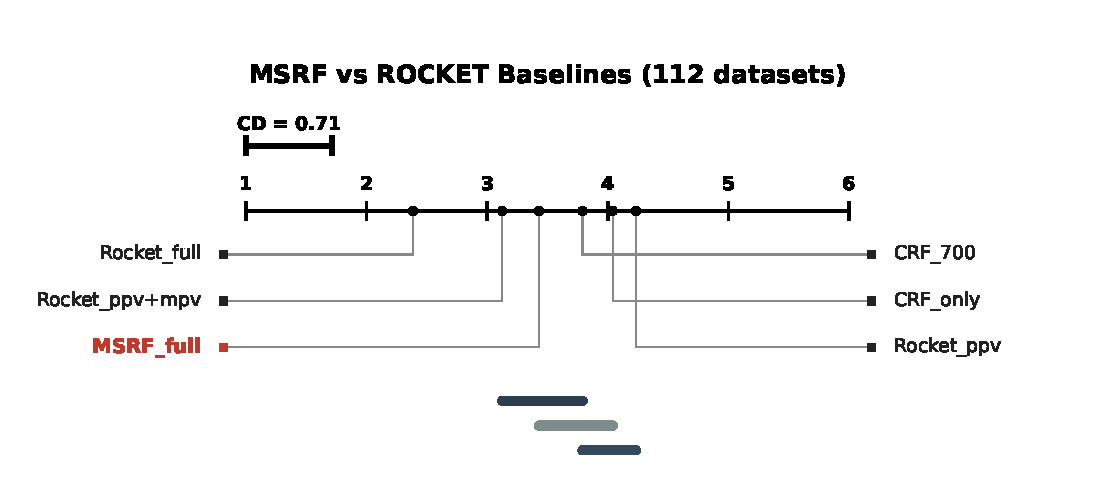
\includegraphics[width=\linewidth]{cd_msrf_vs_rocket.pdf}
  \caption{Critical difference diagram comparing MSRF\textsubscript{full} (1{,}410 dims) against ROCKET baselines and convolutional-only configurations (112 datasets). MSRF\textsubscript{full} achieves a competitive rank despite using 7--43$\times$ fewer features than the ROCKET variants.}
  \label{fig:cd_msrf_vs_rocket}
\end{figure}

\subsection{Timing}

Feature extraction is fast on GPU for all configurations.
For a typical UCR dataset ($T{\approx}300$, $N{\approx}400$):

\begin{table}[h]
  \caption{Typical extraction and classification times (GPU feature extraction, CPU Ridge).}
  \label{tab:timing}
  \centering
  \small
  \begin{tabular}{@{}lc@{}}
    \toprule
    Component & Time \\
    \midrule
    TRF (200 features) & ${<}0.01$s \\
    GRF (10 features) & ${<}0.02$s \\
    SRF (200 features) & ${<}0.01$s \\
    CRF (500 kernels) & ${\sim}0.3$s \\
    Full MSRF\textsubscript{full} pipeline & ${\sim}0.8$s \\
    \bottomrule
  \end{tabular}
\end{table}

The full pipeline---feature extraction plus Ridge classification---completes in under 1~second per dataset for typical UCR sizes.
By contrast, Rocket\textsubscript{full} (60{,}000~dims) requires 1--50\,s for Ridge classification alone due to the much larger feature matrix.

\subsection{Per-Dataset Analysis}

Examining where MSRF features help most reveals a consistent pattern.
Table~\ref{tab:top_improvements} lists the 10 datasets with the largest accuracy gains when augmenting Rocket\textsubscript{ppv} with 410~MSRF features.

\begin{table}[h]
  \caption{Top 10 accuracy improvements from Rocket\textsubscript{ppv} $\to$ Rocket\textsubscript{ppv}+MSRF, and the 5 largest losses.}
  \label{tab:top_improvements}
  \centering
  \small
  \begin{tabular}{@{}lclc@{}}
    \toprule
    Dataset (gain) & $\Delta$Acc & Dataset (loss) & $\Delta$Acc \\
    \midrule
    SyntheticControl     & +0.150 & Herring                    & $-$0.063 \\
    ShapeletSim          & +0.094 & Beef                       & $-$0.033 \\
    Worms                & +0.091 & Haptics                    & $-$0.007 \\
    EOGVerticalSignal    & +0.086 & ProximalPhalanxTW          & $-$0.005 \\
    PigArtPressure       & +0.058 & PhalangesOutlinesCorrect   & $-$0.005 \\
    SemgHandMovementCh2  & +0.051 & & \\
    BeetleFly            & +0.050 & & \\
    CinCECGTorso         & +0.044 & & \\
    ElectricDevices      & +0.032 & & \\
    PowerCons            & +0.028 & & \\
    \bottomrule
  \end{tabular}
\end{table}

The gains are concentrated on datasets where \textbf{positional structure matters} (EOG signals, ECG recordings) or where \textbf{distributional properties differ between classes} (SyntheticControl, ShapeletSim).
The losses are few and small in magnitude---the largest (Herring, $-$0.063) involves a dataset with only 20 training samples where the additional features likely introduce noise.
Across all 112~datasets the mean improvement is positive, confirming that the multi-space signal is beneficial on aggregate.


%==============================================================================
\section{Discussion}
\label{sec:discussion}
%==============================================================================

\textbf{Why does distributing features across spaces help?}
Convolutional features are powerful but live in a single high-dimensional space.
The other three feature types access information that convolutions extract only indirectly---a convolution would need to conspire across many timesteps to approximate a global mean, and would need many kernels at many dilations to replicate a position-specific query.
GRFs are particularly efficient: a single $D$-dimensional projection yields two features that capture global sequence geometry, something that would require thousands of coordinated convolutional kernels.
The experimental evidence confirms this: adding 410~non-convolutional features to 10{,}000 MiniRocket features yields near-universal improvement (67/112~wins).
If TRF+GRF+SRF were redundant with CRF, the Ridge classifier would assign them zero weight.

\textbf{Complementarity saturates with convolutional budget.}
The benefit of MSRF features diminishes as the convolutional budget increases (Table~\ref{tab:complementarity}).
At 60{,}000~features, the massive convolutional set already captures most accessible signal through brute-force coverage.
This suggests a practical guideline: MSRF is most valuable when the convolutional budget is moderate (as in MiniRocket), which is also the regime of greatest practical interest for deployment.

\textbf{Moment pooling vs.\ full embedding.}
We pool GRF embeddings to 2~scalars rather than using the full $D$-dimensional vector.
Ridge regression on a concatenation of heterogeneous features benefits from balanced dimensionality across groups---2~GRF features alongside 1{,}000~CRF features are weighted fairly, whereas 256~GRF features would dominate the Ridge solution.
The mean and std are sufficient statistics for the first two moments of the kernel mean embedding.

\textbf{Limitations.}
TRFs assume absolute position carries information; for truly position-invariant tasks they provide limited value.
GRFs treat the series as an unstructured vector and do not exploit temporal locality.
SRFs require choosing which summary statistics to compute.
The optimal allocation ratio likely varies across datasets; we use a fixed ratio as a robust default.


%==============================================================================
\section{Related Work}
\label{sec:related}
%==============================================================================

\textbf{Random feature methods for TSC.}
ROCKET~\citep{dempster2020rocket} introduced random convolutional kernels for TSC.
MiniRocket~\citep{dempster2021minirocket} uses deterministic PPV-only features.
MultiRocket~\citep{tan2022multirocket} adds multiple pooling statistics.
HYDRA~\citep{dempster2023hydra} introduces competing kernel groups.
All operate exclusively in the convolutional space; MSRF is the first to distribute random features across multiple representation spaces.

\textbf{Random Kitchen Sinks.}
\citet{rahimi2007random,rahimi2008weighted} introduced random Fourier features for kernel approximation.
Extensions include Fastfood~\citep{le2013fastfood} for structured projections and random features for non-stationary kernels~\citep{ton2018spatial}.
Our GRFs apply RKS to the full time series with a novel moment-pooled readout; our SRFs apply random projections to the summary statistic space.

\textbf{Positional encoding and attention.}
Sinusoidal positional encodings~\citep{vaswani2017attention} and Gaussian attention alignment~\citep{luong2015effective,graves2013generating} relate to TRFs, but TRFs are random features for a positional kernel rather than learned attention weights.

\textbf{Shapelet and summary statistic methods.}
Shapelets~\citep{ye2009shapelets} are position-specific pattern matchers; TRFs can be viewed as soft, continuous shapelets.
Catch22~\citep{lubba2019catch22} and TSFresh~\citep{christ2018tsfresh} extract summary statistics; our SRFs go beyond by applying random projections to capture \emph{interactions} between statistics.

\textbf{Wavelet scattering.}
TRF with multiple scales resembles a Gabor filter bank~\citep{mallat2012group}, but captures level rather than frequency.


%==============================================================================
\section{Conclusion}
\label{sec:conclusion}
%==============================================================================

We introduced Multi-Space Random Features (MSRF), a framework that distributes random features across temporal, global, statistical, and convolutional spaces for time series classification.
On the full 112-dataset UCR archive, appending just 410~non-convolutional MSRF features to MiniRocket improves accuracy on 67~datasets with only 14~losses.
At a fixed feature budget (${\sim}$1{,}400 dimensions), multi-space allocation outperforms a purely convolutional baseline on a majority of datasets, confirming that diversity across representation spaces is more effective than scale within a single space.
MSRF\textsubscript{full} with 1{,}410 features achieves higher mean accuracy than MiniRocket with 10{,}000 features.
The framework is simple, fast, requires no learned parameters beyond the Ridge classifier, and serves as a drop-in complement to existing ROCKET pipelines.
A notable contribution is moment-pooled Random Fourier Features, which compresses a high-dimensional random Fourier embedding into two scalar features capturing global signal geometry---a construction that, to our knowledge, is novel in the random features literature.


\bibliographystyle{plainnat}
\bibliography{references}


%==============================================================================
\newpage
\appendix
\section{Implementation Details}
\label{app:implementation}
%==============================================================================

All feature extractors are implemented as \texttt{torch.nn.Module} subclasses for GPU execution.
Random parameters (Gaussian centers, projection matrices, etc.) are drawn once at initialization and frozen.
The full implementation, including all feature extractors, evaluation scripts, and reproduction instructions, is available at \url{https://anonymous.4open.science/r/msrf/}.

\subsection{Temporal Random Feature Computation}

\begin{algorithmic}
\REQUIRE Time series batch $\mathbf{X} \in \mathbb{R}^{N \times T}$, number of features $K_T$, seed
\STATE Sample $\mu_k \sim \mathrm{Uniform}[0, T]$, $\sigma_k \sim \mathrm{LogUniform}[1, T/2]$ for $k = 1, \ldots, K_T$
\STATE Construct weight matrix $W_{kt} = \exp(-(t - \mu_k)^2 / (2\sigma_k^2))$, \quad $W \in \mathbb{R}^{K_T \times T}$
\STATE \textbf{return} $\mathbf{X} W^\top \in \mathbb{R}^{N \times K_T}$ \COMMENT{single matrix multiply}
\end{algorithmic}

\subsection{Global Random Feature Computation}

\begin{algorithmic}
\REQUIRE Time series batch $\mathbf{X} \in \mathbb{R}^{N \times T}$, $n_{\mathrm{proj}}$ projections, embedding dim $D$
\FOR{$i = 1, \ldots, n_{\mathrm{proj}}$}
  \STATE Sample $W_i \in \mathbb{R}^{T \times D}$ with entries $\sim \mathcal{N}(0, 1/T)$, $\mathbf{b}_i \sim \mathrm{Uniform}[0, 2\pi]^D$
  \STATE $\mathbf{Z}_i = \cos(\mathbf{X} W_i + \mathbf{b}_i) \in \mathbb{R}^{N \times D}$
  \STATE Extract $\mathrm{mean}(\mathbf{Z}_i, \mathrm{dim}{=}1)$ and $\mathrm{std}(\mathbf{Z}_i, \mathrm{dim}{=}1)$ \COMMENT{two features per projection}
\ENDFOR
\STATE \textbf{return} Concatenation of all mean/std features $\in \mathbb{R}^{N \times 2n_{\mathrm{proj}}}$
\end{algorithmic}

\subsection{Statistical Random Feature Computation}

\begin{algorithmic}
\REQUIRE Time series batch $\mathbf{X} \in \mathbb{R}^{N \times T}$, number of features $K_S$
\STATE Compute $M$-dimensional summary statistics: mean, std, skew, kurtosis, lag-1 autocorrelation, min, max, median, IQR
\STATE $\mathbf{S} \in \mathbb{R}^{N \times M}$
\FOR{$k = 1, \ldots, K_S$}
  \STATE Sample $W_k \in \mathbb{R}^{d \times M}$, $\mathbf{b}_k \in \mathbb{R}^d$, $\mathbf{u}_k \in \mathbb{R}^d$
  \STATE $\phi_k = \mathbf{u}_k^\top \mathrm{ReLU}(W_k \mathbf{S}^\top + \mathbf{b}_k) \in \mathbb{R}^N$ \COMMENT{two-layer random network}
\ENDFOR
\STATE \textbf{return} $[\phi_1, \ldots, \phi_{K_S}]^\top \in \mathbb{R}^{N \times K_S}$
\end{algorithmic}

\subsection{Convolutional Random Feature Computation}

CRF extraction follows MiniRocket~\citep{dempster2021minirocket}.
Random kernels of length 9 with binary weights from $\{-1, 2\}$ are applied at multiple dilations $\{1, 2, 4, \ldots, 2^{\lfloor\log_2(T/8)\rfloor}\}$.
Each kernel-dilation pair produces PPV (proportion of positive values) and max pooling features.
Our GPU implementation processes all kernels in a single batched convolution.

\subsection{Full Pipeline}

\begin{algorithmic}
\REQUIRE Training set $(\mathbf{X}_{\mathrm{train}}, \mathbf{y}_{\mathrm{train}})$, test set $\mathbf{X}_{\mathrm{test}}$
\STATE Initialize TRF, GRF, SRF, CRF extractors with fixed random seed
\STATE $\Phi_{\mathrm{train}} = [\mathrm{TRF}(\mathbf{X}),\; \mathrm{GRF}(\mathbf{X}),\; \mathrm{SRF}(\mathbf{X}),\; \mathrm{CRF}(\mathbf{X})]$ for $\mathbf{X} = \mathbf{X}_{\mathrm{train}}$
\STATE Standardize $\Phi_{\mathrm{train}}$ to zero mean, unit variance; apply same transform to $\Phi_{\mathrm{test}}$
\STATE Fit \texttt{RidgeClassifierCV} on $(\Phi_{\mathrm{train}}, \mathbf{y}_{\mathrm{train}})$
\STATE \textbf{return} Predictions on $\Phi_{\mathrm{test}}$
\end{algorithmic}


%==============================================================================
\section{Additional Critical Difference Diagrams}
\label{app:cd_diagrams}
%==============================================================================

\begin{figure}[h]
  \centering
  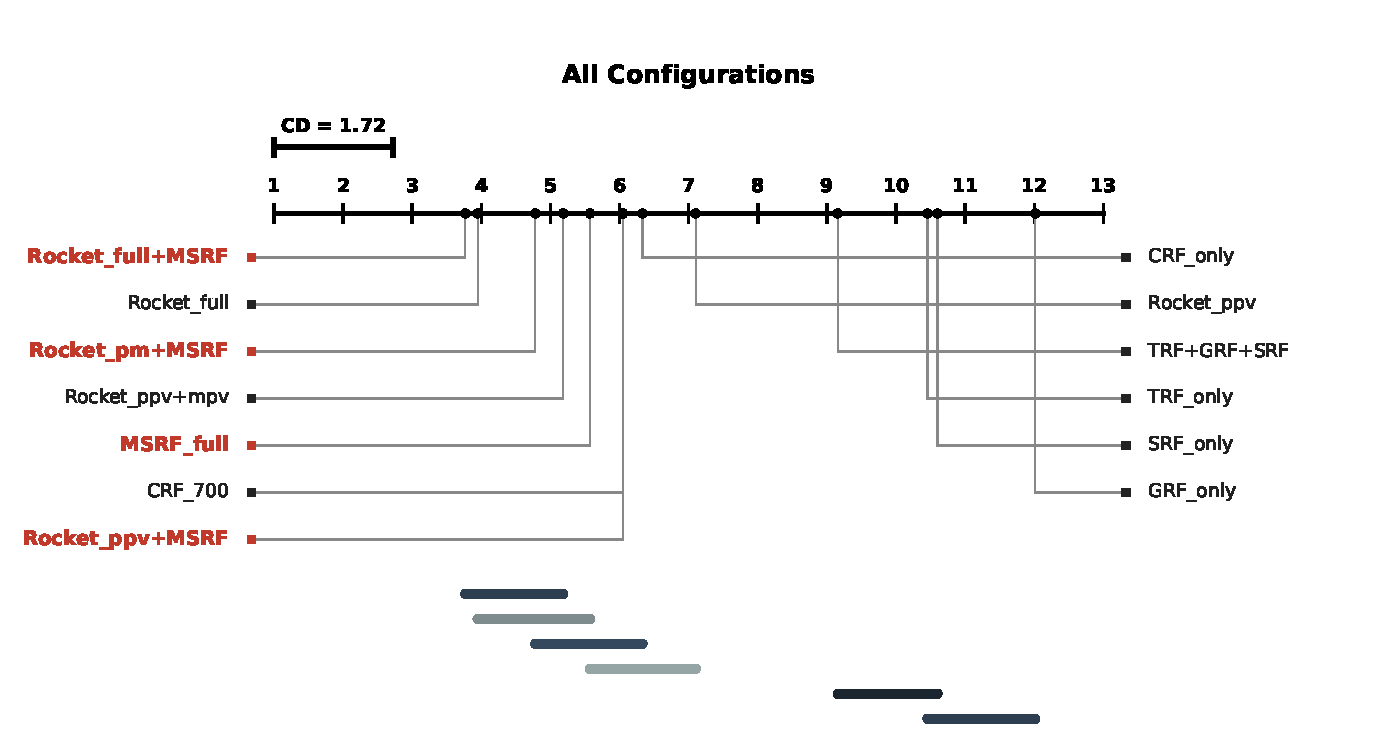
\includegraphics[width=\linewidth]{cd_diagram_full.pdf}
  \caption{Critical difference diagram for all 13 configurations (112 UCR datasets, Nemenyi test at $\alpha{=}0.05$). MSRF-augmented variants (red labels) consistently rank higher than their non-augmented counterparts. The individual non-convolutional spaces (TRF, GRF, SRF) rank lowest, confirming that their value lies in combination.}
  \label{fig:cd_full}
\end{figure}

\begin{figure}[h]
  \centering
  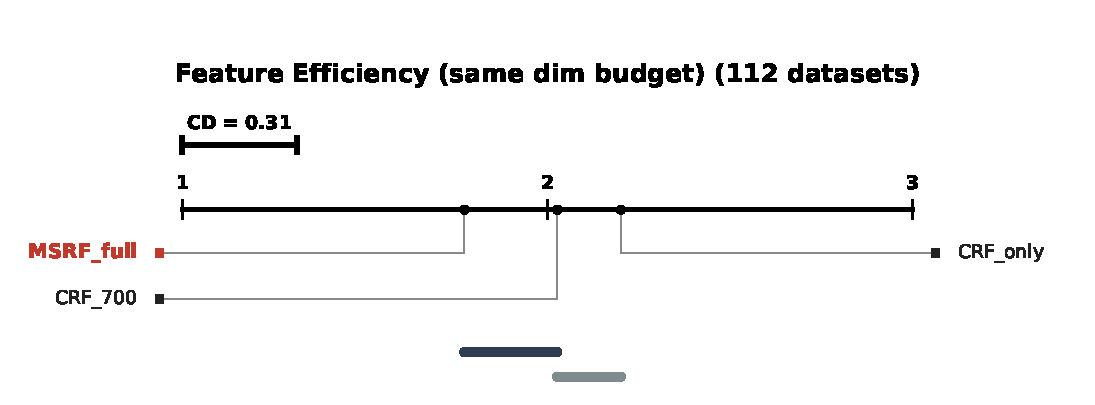
\includegraphics[width=\linewidth]{cd_feature_efficiency.pdf}
  \caption{Critical difference diagram for the feature efficiency comparison (112 datasets). MSRF\textsubscript{full} (500 conv + 410 non-conv = 1{,}410 dims), CRF\textsubscript{700} (700 conv $\times$ 2 = 1{,}400 dims), and CRF\textsubscript{only} (500 conv $\times$ 2 = 1{,}000 dims). At a matched dimensionality budget, multi-space allocation ranks first.}
  \label{fig:cd_efficiency}
\end{figure}


\end{document}
